\documentclass[14pt,a4paper]{extarticle}

\usepackage{fontspec}
\setmainfont{Times New Roman}
\setsansfont{Arial}
\setmonofont{Courier New}[Scale=MatchLowercase]

\usepackage[
  a4paper,
  left=25mm,
  right=20mm,
  top=20mm,
  bottom=20mm,
  headheight=17pt,
  headsep=7mm,
  footskip=10mm
]{geometry}

\usepackage{setspace}
\setstretch{1.5}
\usepackage{indentfirst}
\setlength{\parindent}{1.25cm}
\setlength{\emergencystretch}{3em}

\usepackage[english]{babel}
\usepackage{csquotes}
\usepackage{xcolor}
\usepackage{xurl}
\usepackage{pdfpages}
\usepackage{enumitem}
\urlstyle{same}

\usepackage[
  colorlinks=true,
  linkcolor=black,
  citecolor=black,
  urlcolor=black
]{hyperref}

\usepackage{fancyhdr}
\pagestyle{fancy}
\fancyhf{}
\fancyhead[R]{\thepage}
\renewcommand{\headrulewidth}{0pt}

\sloppy

\begin{document}

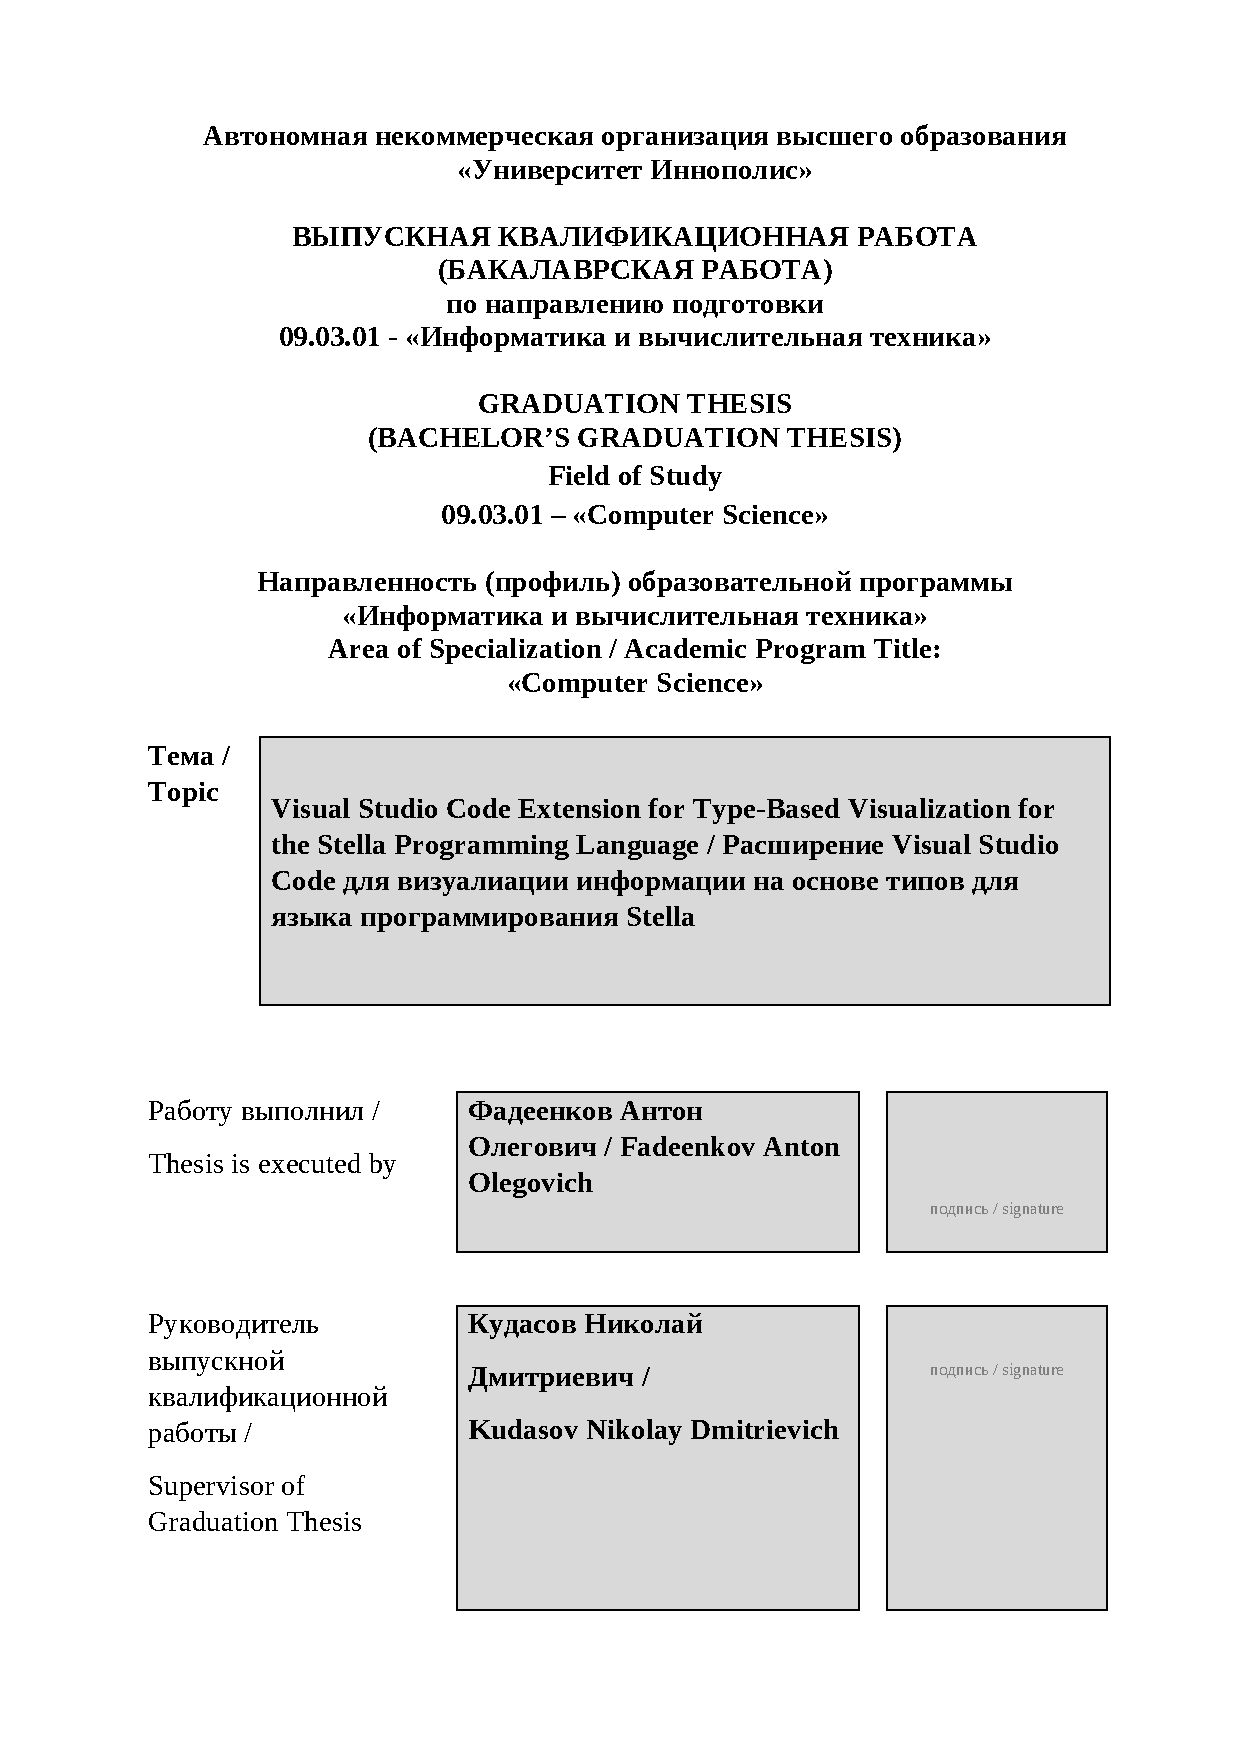
\includepdf[pages=1, pagecommand={\thispagestyle{empty}}]{title.pdf}
\setcounter{page}{2}

\section*{Introduction, Goal and Tasks}

The graduation thesis is devoted to the development of a Visual Studio Code extension for visualizing syntax and type-analysis results for programs written in Stella. Stella is an educational statically typed language used for studying type systems and compiler construction. In such courses, it is important to see not only the final error or inferred type, but also intermediate analysis structures: the abstract syntax tree, the typing context, the type-derivation tree, and dependencies between expressions.

The problem is that standard editor support usually shows only the final output of the language server: a hover, an underlined error, or a short diagnostic message. As a result, the student has to reconstruct which subexpressions participated in checking and why a judgment of the form $\Gamma \vdash e : T$ was obtained, where $\Gamma$ denotes the typing context, $e$ is an expression, and $T$ is its type.

The goal of the work is to design and implement a Visual Studio Code extension that presents Stella analysis results as interactive views linked to source code. To achieve this goal, the work studies educational visualization, defines the required views, designs communication between the client and the language server, implements custom Language Server Protocol requests, and validates the prototype through functional scenarios.

\section*{Literature Review}

Program visualization is used in computer science education to explain structures and processes that are difficult to observe directly. Studies of software visualization and algorithm visualization show that interactive representations may support understanding of abstract processes, but their results cannot be transferred automatically to a specific new tool without separate validation. Therefore, the works by Price, Hundhausen, Naps, Sorva, and Kogan are used as a design background rather than as direct evidence of the effectiveness of the extension.

Related tools include Jeliot and visAST. Jeliot visualizes program execution, while visAST links source text with an abstract syntax tree. The difference of this work is that the developed extension covers not only syntax but also type-related information: the typing context, the derivation tree, the error trace, and the dependency graph. The theoretical basis is formed by work on static type systems, typing judgments, and program analysis.

\section*{Brief Description of the Thesis Content}

The work develops a prototype Visual Studio Code extension for Stella. The client side implements editor views, while the server side prepares analysis data and transfers it through extended Language Server Protocol requests. JSON-RPC is used for communication, which is consistent with the LSP architecture and separates the computation of analysis results from their presentation in the user interface.

The main results are five views. AST View shows the program structure as a tree. Scope View displays scope information and the typing context. Type Derivation View shows the sequence of applied typing rules. Type Error Trace View helps trace the path to a type error. Type Dependency Graph shows dependencies between expressions and typing judgments; this view is related to the ideas of program dependence graph and program slicing, but is adapted to the educational Stella language.

Special attention is paid to the consistency between the technology stack and design principles. TypeScript is chosen as the main implementation language because of static typing and compatibility with the Visual Studio Code ecosystem. Langium is used for language infrastructure, and the Visual Studio Code API is used for Tree View and Webview interfaces. This stack preserves the connection between analysis, editor integration, and the user interface without a separate external application.

The result is validated functionally: the work considers representative Stella programs, correctness of language-server responses, and presentation of results in the editor interface. A full user study was not conducted, so conclusions about usability and influence on understanding are limited. This limitation is explicitly treated as a threat to the validity of the results.

\section*{Conclusion}

As a result, the work created a Visual Studio Code extension that visualizes intermediate analysis results for Stella programs. The extension shows not only the final checking result, but also the structures involved in syntax and type analysis. This makes the prototype useful as a supporting tool for studying type-system implementation.

The main contribution of the work is the design of Stella-specific views, implementation of data exchange between the extension and the language server, creation of the Visual Studio Code user interface, and functional validation of the prototype. Further development may include a full user study, usability evaluation using SUS, improvement of graph visualization, and support for new Stella language constructs.
\section*{References}

\begin{enumerate}[label={[\arabic*]},leftmargin=*,itemsep=0pt,topsep=0pt]
\item Microsoft. Language Server Protocol Specification 3.17. URL: \url{https://microsoft.github.io/language-server-protocol/specifications/lsp/3.17/specification/}.
\item JSON-RPC Working Group. JSON-RPC 2.0 Specification. URL: \url{https://www.jsonrpc.org/specification}.
\item Microsoft. Visual Studio Code Extension API. URL: \url{https://code.visualstudio.com/api}.
\item Microsoft. Visual Studio Code Tree View API. URL: \url{https://code.visualstudio.com/api/extension-guides/tree-view}.
\item Microsoft. Visual Studio Code Webview API. URL: \url{https://code.visualstudio.com/api/extension-guides/webview}.
\item TypeFox. Langium Documentation. URL: \url{https://langium.org/docs/}.
\item Kudasov N. Stella Language Documentation. URL: \url{https://fizruk.github.io/stella/site/core/introduction/}.
\item Abounegm A., Kudasov N., Stepanov A. Teaching Type Systems Implementation with STELLA. 2024. URL: \url{https://arxiv.org/abs/2407.08089}.
\item Pierce B. C. Types and Programming Languages. MIT Press, 2002.
\item Harper R. Practical Foundations for Programming Languages. Cambridge University Press, 2016.
\item Nielson F., Nielson H. R., Hankin C. Principles of Program Analysis. Springer, 1999.
\item Price B. A., Baecker R. M., Small I. S. A Principled Taxonomy of Software Visualization // Journal of Visual Languages and Computing. 1993.
\item Hundhausen C. D., Douglas S. A., Stasko J. T. A Meta-Study of Algorithm Visualization Effectiveness // Journal of Visual Languages and Computing. 2002.
\item Naps T. L. et al. Exploring the Role of Visualization and Engagement in Computer Science Education // ITiCSE Working Group Reports. 2002.
\item Sorva J., Karavirta V., Malmi L. A Review of Generic Program Visualization Systems // ACM Transactions on Computing Education. 2013.
\item Moreno A., Myller N., Sutinen E., Ben-Ari M. Visualizing Programs with Jeliot 3 // AVI. 2004.
\item Aalvik R. visAST: Generic AST Visualiser for Software Language Education: master's thesis. University of Bergen, 2019.
\item Ferrante J., Ottenstein K. J., Warren J. D. The Program Dependence Graph and Its Use in Optimization // ACM TOPLAS. 1987.
\item Brooke J. SUS: A Quick and Dirty Usability Scale // Usability Evaluation in Industry. Taylor \& Francis, 1996.
\item Bangor A., Kortum P., Miller J. Determining What Individual SUS Scores Mean // Journal of Usability Studies. 2009.
\item Wohlin C. et al. Experimentation in Software Engineering. Springer, 2012.
\item Runeson P., Hoest M. Guidelines for Conducting and Reporting Case Study Research in Software Engineering // Empirical Software Engineering. 2009.
\end{enumerate}

\end{document}



